\begin{thmBox}{32.1}[thm:32.1]
    Every regular space with a countable basis is normal.

    \baseRule

    \begin{proofBox}
        Let \( X \) be a regular space with a countable basis \( \mathcal{B} \). 
        Let \( A \) and \( B \) be disjoint closed subsets of \( X \).
        We want to show that there exists disjoint open sets containing \( A \) and 
        \( B \).
        Using the regularity of \( X \), we see that for each \( x \in A \), there 
        exists disjoint open sets \( U_{ x } \) and \( W_{ x } \) that contain \( x \) 
        and \( B \),
        respectively.
        By [\hyperlink{lem:31.1}{Lemma 31.1}], we see that there exists an open 
        neighborhood \( V_{ x } \) of \( x \) such that 
        \( \mathrm{Cl} \ V_{ x } \subset U_{ x } \).
        Furthermore, since \( X \) is generated by the basis \( \mathcal{B} \), we see 
        that there exists a basis element \( B_{ x } \in \mathcal{B} \) such that 
        \( x \in B_{ x } \subset V \) -- notice that \( B_{ x } \) could be the 
        same for multiple \( x \in A \).
        By choosing such a basis element for each \( x \in A \), we see that 
        \( \{ B_{ x } \}_{ x \in A } \) is a countable covering of \( A \) whose closures do not intersect \( B \): it is countable as 
        \( \{ B_{ x } \}_{ x \in A } \) must be a subcollection of a countable set, 
        which must still be countable; and, we see for each \( x \in A \) that 
        \( B_{ x } \subset V_{ x } \), which implies that 
        \( \overline{ B }_{ x } \subset \overline{ V }_{ x } \subset U_{ x } \),
        with each \( U_{ x } \) being disjoint from \( B \).
        Since this covering of \( A \) is countable, we can index it with the 
        positive integers; let us denote it by 
        \( \{ U_{ n } \}_{ n \in \mathbb{Z}_{ + } } \).

        \baseSkip

        Similarly, we can choose a countable collection 
        \( \{ V_{ n } \}_{ n \in \mathbb{Z}_{ + } } \) of open sets covering \( B \),
        such that each set \( \overline{ V }_{ n } \) is disjoint from \( A \).
        The sets \( U = \bigcup_{ n \in \mathbb{Z}_{ + } } U_{ n } \)
        \( V = \bigcup_{ n \in \mathbb{Z}_{ + } } V_{ n } \) are open sets containing 
        \( A \) and \( B \), respectively, but they need not be disjoint. 
        We perform the following simple trick to construct two open sets that are 
        disjoint. 
        Given \( n \), we define 
        \begin{equation*}
            U_{ n }' 
            = 
            U_{ n } \setminus 
            \left( \bigcup_{ i = 1 }^{ n } \overline{ V }_{ i } \right)
            \quad \mathrm{and} \quad 
            V_{ n }' 
            = 
            V_{ n } \setminus 
            \left( \bigcup_{ i = 1 }^{ n } \overline{ U }_{ i } \right)
        \end{equation*}
        Note that each set \( U_{ n }' \) is open, being the difference of an open set 
        \( U_{ n } \) and a closed set 
        \( \bigcup_{ i = 1 }^{ n } \overline{ V }_{ i } \).
        Similarly, each set \( V_{ n }' \) is open.
        The collection \( \{ U_{ n }' \}_{ n \in \mathbb{Z}_{ + } } \) covers \( A \)
        because each \( x \in A \) belongs to \( U_{ n } \) for some \( n \), and we 
        have that \( x \) belongs to \textit{none} of the sets 
        \( \overline{ V }_{ i } \). 
        Similarly, the collection \( \{ V_{ n }' \}_{ n \in \mathbb{Z}_{ + } } \) 
        covers \( B \).

        \begin{figure}[H]
            \centering
            \begin{minipage}{ 0.45\linewidth }
                \centering 
                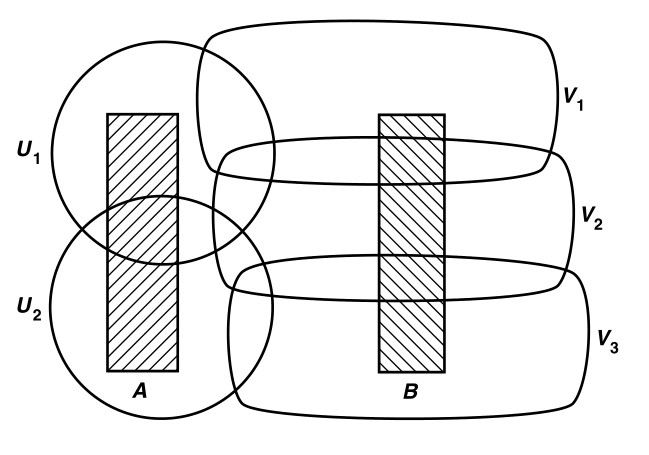
\includegraphics[ width = 0.95\linewidth ]{figures/Section 32/32-1.jpg}
            \end{minipage}
            \begin{minipage}{ 0.45\linewidth }
                \centering 
                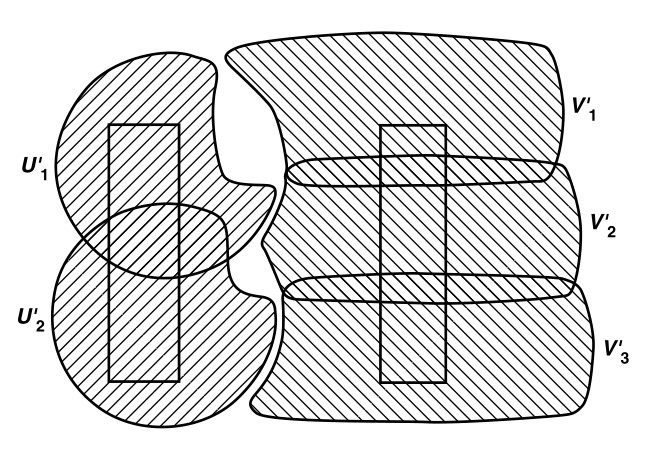
\includegraphics[ width = 0.95\linewidth ]{figures/Section 32/32-2.jpg}
            \end{minipage}
            \caption{A visual on the constructed covers}
            \label{fig:32-1}
        \end{figure}

        Finally, the open sets 
        \begin{equation*}
            U'
            =
            \bigcup_{ n \in \mathbb{Z}_{ + } } U_{ n }'
            \quad \mathrm{and} \quad 
            V'  
            =
            \bigcup_{ n \in \mathbb{Z}_{ + } } V_{ n }'
        \end{equation*}
        are disjoint. 
        For if \( x \in U' \cap V' \), then we see that 
        \( x \in U_{ j }' \cap V_{ k }' \) for some \( j \) and \( k \).
        Suppose that \( j \leq k \). 
        It follows from the definition of \( U_{ j }' \) that \( x \in U_{ j } \);
        and since \( j \leq k \), it follows from the definition of \( V_{ k }' \)
        that \( x \notin \overline{ U }_{ j } \).
        A similar contradiction arises if \( j \geq k \).
    \end{proofBox}
\end{thmBox}

\begin{thmBox}{Variation of [\hyperlink{thm:32.1}{Theorem 32.1}]}[thm:32.1-v]
    Let \( X \) be regular and Lindel\"{o}f.
    Then \( X \) is normal.

    \baseRule

    \begin{proofBox}
        Let \( X \) be regular and Lindel\"{o}f.
        Let \( A \) and \( B \) be disjoint and closed in \( X \).
        We claim that there exists an open cover \( \mathcal{U} \) of \( A \) such that,
        for all \( U \in \mathcal{U} \), we have that 
        \( \overline{ U } \cap B = \emptyset \).
        Likewise, we further claim that there exists an open cover \( \mathcal{V} \)
        of \( B \) such that, for all \( V \in \mathcal{V} \), we have that
        \( \overline{ V } \cap A = \emptyset \).

        \baseSkip

        To show why, we have that for all \( a \in A \), \( X \setminus B \) is an
        open neighborhood of \( a \) in \( X \).
        By [\hyperlink{lem:31.1}{Lemma 31.1}], we see that there exists an neighborhood 
        \( U_{ a } \) of \( a \)  such that 
        \( \overline{ U_{ a } } \subset X \setminus B \).
        Thus, we see that \( \overline{ U_{ a } } \cap B = \emptyset \).
        Let \( \mathcal{U} = \{ U_{ a } \mid a \in A \} \).
        Likewise, we can construct the desired \( \mathcal{V} \) the same way.

        \baseSkip

        Since \( A \) and \( B \) are closed and \( X \) is Lindel\"{o}f, we have that 
        \( \mathcal{U} \) and \( \mathcal{V} \) both admit countable subcovers by 
        [\hyperlink{thm:30.5}{Variation of Theorem 30.2}].
        We shall denote them to be as follows:
        \begin{equation*}
            \{ U_{ i } \mid i \in \mathbb{Z}_{ + } \}
            \quad \mathrm{and} \quad 
            \{ V_{ i } \mid i \in \mathbb{Z}_{ + } \}
        \end{equation*}
        where 
        \begin{equation*}
            \overline{ U_{ i } } \cap B = \emptyset
            \quad \mathrm{and} \quad 
            \overline{ V_{ i } } \cap A = \emptyset
            \quad \forall i \in \mathbb{Z}_{ + }
        \end{equation*}
        We define new open covers
        \begin{equation*}
            \begin{aligned}
                \tilde{U}_{ 1 }
                &=
                U_{ 1 } \setminus \overline{ V_{ 1 } }
                \\ 
                \tilde{U}_{ 2 }
                &=
                U_{ 2 } \setminus ( \overline{ V_{ 1 } } \cup \overline{ V_{ 2 } } )
                \\ 
                &\vdots
                \\
                \tilde{U}_{ n }
                &=
                U_{ n } \setminus 
                \left( \bigcup_{ j = 1 }^{ n } \overline{ V_{ j } } \right)
            \end{aligned}
            \quad \mathrm{and} \quad 
            \begin{aligned}
                \tilde{V}_{ 1 }
                &=
                V_{ 1 } \setminus \overline{ U_{ 1 } }
                \\
                \tilde{V}_{ 2 }
                &=
                V_{ 2 } \setminus ( \overline{ U_{ 1 } } \cup \overline{ U_{ 2 } } )
                \\ 
                &\vdots
                \\
                \tilde{V}_{ n }
                &=
                V_{ n } \setminus 
                \left( \bigcup_{ j = 1 }^{ n } \overline{ U_{ j } } \right)
            \end{aligned}
        \end{equation*}
        Notice that for each \( n \), we have that 
        \( \bigcup_{ j = 1 }^{ n } \overline{ U_{ j } } \) and
        \( \bigcup_{ j = 1 }^{ n } \overline{ V_{ j } } \)
        are both closed in \( X \) as they are a finite union of closed sets. 
        We now set
        \begin{equation*}
            U
            =
            \bigcup_{ i = 1 }^{ \infty } \tilde{U}_{ i }
            \quad \mathrm{and} \quad 
            V
            =
            \bigcup_{ j = 1 }^{ \infty } \tilde{V}_{ j }
        \end{equation*}
        which we see are disjoint open neighborhoods of \( A \) and \( B \).
    \end{proofBox}
\end{thmBox}

\begin{thmBox}{32.2}[thm:32.2]
    Every metrizable space is normal.

    \baseRule

    \begin{proofBox}
        Let \( X \) be a metric space with metric \( d \).
        We have already seen metric spaces be Hausdorff.
        Let disjoint closed subsets \( C, D \) in \( X \) be given.
        Because we have that \( X \setminus D \) is open, we have for all
        \( c \in C \), there exists \( r_{ c } > 0 \) so that 
        \begin{equation*}
            B_{ r_{ c } }( c ) \subset X \setminus D
        \end{equation*}
        Likewise, because \( X \setminus C \) is open, we have for all
        \( d \in D \), there exists \( r_{ d } > 0 \) so
        \begin{equation*}
            B_{ r_{ d } }( d ) \subset X \setminus C    
        \end{equation*}
        Let \( U = \bigcup_{ c \in C } B_{ \frac{ r_{ c } }{ 2 } }( c ) \) and
        \( V = \bigcup_{ d \in D } B_{ \frac{ r_{ d } }{ 2 } }( d ) \).
        Notice that \( U \) and \( V \) are still open neighborhoods of
        \( C \) and \( D \), respectively.
        We want to show that \( U \cap V = \emptyset \).

        \baseSkip

        Towards a contradiction, let us suppose that
        \( U \cap V \neq \emptyset \).
        Then, there exists some \( p \in U \cap V \).
        Furthermore, there exists some \( c \in C \) and \( d \in D \) such that
        \( p \in B_{ \frac{ r_{ c } }{ 2 } }( c ) \cap B_{ \frac{ r_{ d } }{ 2 } }( d ) \).
        The triangle inequality implies that 
        \begin{equation*}
            d( c, d )
            \leq 
            d ( c, p ) + d(  p, d )
            < \frac{ r_{ c } }{ 2 } + \frac{ r_{ d } }{ 2 }
        \end{equation*}
        Thus us now look at two possible cases:

        \baseSkip
        \wrapBox{Case 1: \( r_{ c } < r_{ d } \)}
        In this case, we see that \( d( c, d ) < r_{ d } \), which tells us that
        \( c \in B_{ r_{ d } }( d ) \), which contradicts the fact
        \( B_{ r_{ d } }( d ) \subset X \setminus C \).

        \baseSkip
        \wrapBox{Case 2: \( r_{ c } > r_{ d } \)}
        In this case, we see that \( d( c, d ) < r_{ c } \), which tells us that
        \( d \in B_{ r_{ c } }( c ) \), which contradicts the fact
        \( B_{ r_{ c } }( c ) \subset X \setminus D \).

        \baseSkip

        Thus, we have that any metric space is Hausdorff.
    \end{proofBox}  
\end{thmBox}

\begin{thmBox}{32.3}[thm:32.3]
    Every compact Hausdorff space is normal.

    \baseRule

    \begin{proofBox}
        Let \( X \) be a compact Hausdorff space.
        Let \( A \) and \( B \) be two disjoint closed sets in \( X \).
        Our goal is to show that there exists disjoint open sets \( K \) and \( L \)
        containing \( A \) and \( B \), respectively. 
        
        \baseSkip

        Since both \( A \) and \( B \) are closed in \( X \), we have that they must be
        compact themselves as \( X \) is compact.
        Hence, by [\hyperlink{thm:26.4}{Theorem 26.4}], we see that there exists 
        disjoint open sets \( K \) and \( L \) containing \( A \) and \( B \), 
        respectively.
    \end{proofBox}
\end{thmBox}

\begin{thmBox}{Variation of [\hyperlink{thm:32.3}{Theorem 32.3}]}[thm:32.3-v]
    Every locally compact Hausdorff space is regular.

    \baseRule

    \begin{proofBox}
        Let \( X \) be locally compact Hausdorff.
        Let disjoint point \( p \in X \) and closed \( C \) of \( X \) be given.
        Since \( C \) is closed, we see that \( X \setminus C \) is open.
        Furthermore, \( X \setminus C \) is an open neighborhood of \( p \).
        Since \( X \) is locally compact, this implies that there exists a 
        compact neighborhood \( K \) of \( p \) in \( X \setminus C \).
        Let \( U = \mathrm{Int} \ K \).
        Notice that \( U \) is still an open neighborhood of \( p \).
        Let \( V = X \setminus K \).
        \( V \) is an open neighborhood of \( C \) because \( K \) is 
        compact, hence closed since \( X \) is Hausdorff.
        As a result, we see that \( U \cap V = \emptyset \).
    \end{proofBox}
\end{thmBox}

\begin{thmBox}{32.4}[thm:32.4]
    Every well-ordered set \( X \) is normal in the order topology.

    \baseRule

    \begin{proofBox}

    \end{proofBox}
\end{thmBox}